
\section{Étude de l'amplitude du déplacement de l'actionneur pour conserver un mouvement naturel} % II 
%\section{Objectif}
\begin{obj}
Déterminer la course des actionneurs permettant de suivre les mouvements du corps conformément à l'exigence Id2 du cahier des charges partiel.
\end{obj}


L'exigence Id2 «~Préserver l'activité musculaire~» est composée de deux exigences Id2.1 et Id2.2 (tableau \ref{ccs_mp_2023_tab_02}). Le fonctionnement de l'exosquelette nécessite une mise en précontrainte. Pour cette mise en précontrainte, chaque actionneur linéaire doit exercer une force de \SI{40}{N}. Cette valeur est obtenue par déplacement vertical de la ceinture haute par rapport à la ceinture basse.

\begin{table}[h]
\begin{center}
\begin{tabular}{|l|p{4cm}|p{4cm}|l|l|}
\hline
Id & Exigence & Critère & Niveau & Flexibilité \\
\hline
Id2.1 & Permettre le mouvement de translation de la ceinture haute par rapport à la ceinture basse & Déplacement vertical $\Delta h$ de la ceinture haute par rapport à la ceinture basse & $\Delta h=50 \mathrm{~mm}$ & < 10 \% \\
\hline
Id2.2 & Permettre le mouvement de rotation de la ceinture haute par rapport à la ceinture basse & Amplitude de rotation $\varphi$ & [ $0,+20^{\circ}$ ] selon l'axe sagittal & < 10 \% \\
\hline
\end{tabular}
%\captionsetup{labelformat=empty}
\caption{\label{ccs_mp_2023_tab_02}Extrait du cahier des charges fonctionnel limité au mouvement dans le plan sagittal de l'exosquelette}
\end{center}
\end{table}

\subsection{Analyse des exigences 2.1 et 2.2} % Ajout XP

L'exigence Id2.1 correspond à la valeur du déplacement vertical nécessaire à la précontrainte. Cette valeur est propre à chaque utilisateur. Dans le cas extrême, cette valeur correspond à un déplacement vertical de \SI{50}{mm}. L'étude cinématique est limitée à un mouvement de flexion avant. La figure \ref{ccs_mp_2023_fig_06} décrit le mouvement ainsi que le positionnement de l'exosquelette dans le plan sagittal. La figure \ref{ccs_mp_2023_fig_07} décrit le modèle géométrique paramétré de l'exosquelette. La liaison sphère-cylindre en $C$ modélise les degrés de liberté supprimés par les éléments extérieurs au système (colonne vertébrale + tissus mous).\\

\question{\label{ccs_mp_2023_q_03}
Déterminer l'expression de la longueur $l_{2}(t)$ en fonction de $\varphi(t), h(t), b$ et $a$.}
\ifprof
\begin{corrige}
\end{corrige}
\else
\fi


%\begin{figure}[h]
%\begin{center}
%  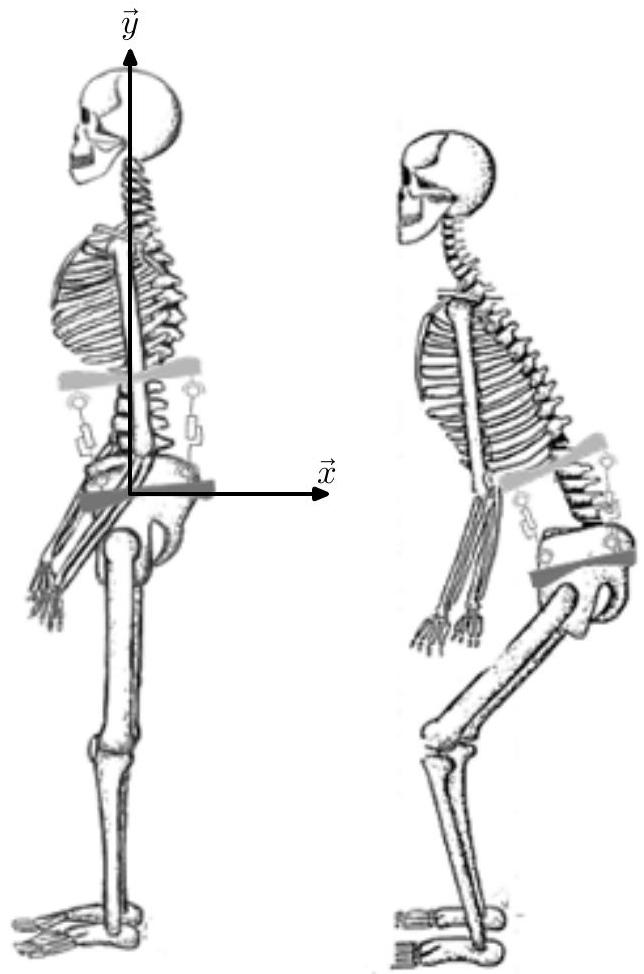
\includegraphics[width=\textwidth]{2025_09_16_5f2d7643f7e649c6833dg-05}
%\captionsetup{labelformat=empty}
%\caption{Figure 6 Mouvement de flexion et implantation de l'exosquelette}
%\end{center}
%\end{figure}


\begin{figure}[!h]
\centering
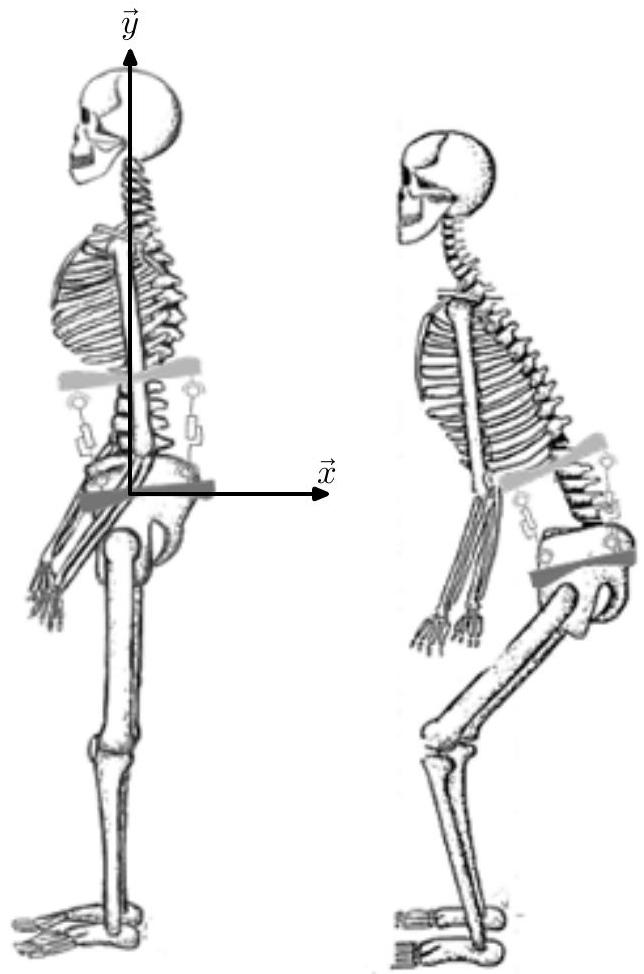
\includegraphics[width=.4\textwidth]{2025_09_16_5f2d7643f7e649c6833dg-05}
\caption{\label{ccs_mp_2023_fig_06}  Mouvement de flexion et implantation de l'exosquelette}
\end{figure}



%\begin{figure}[h]
%\begin{center}
%  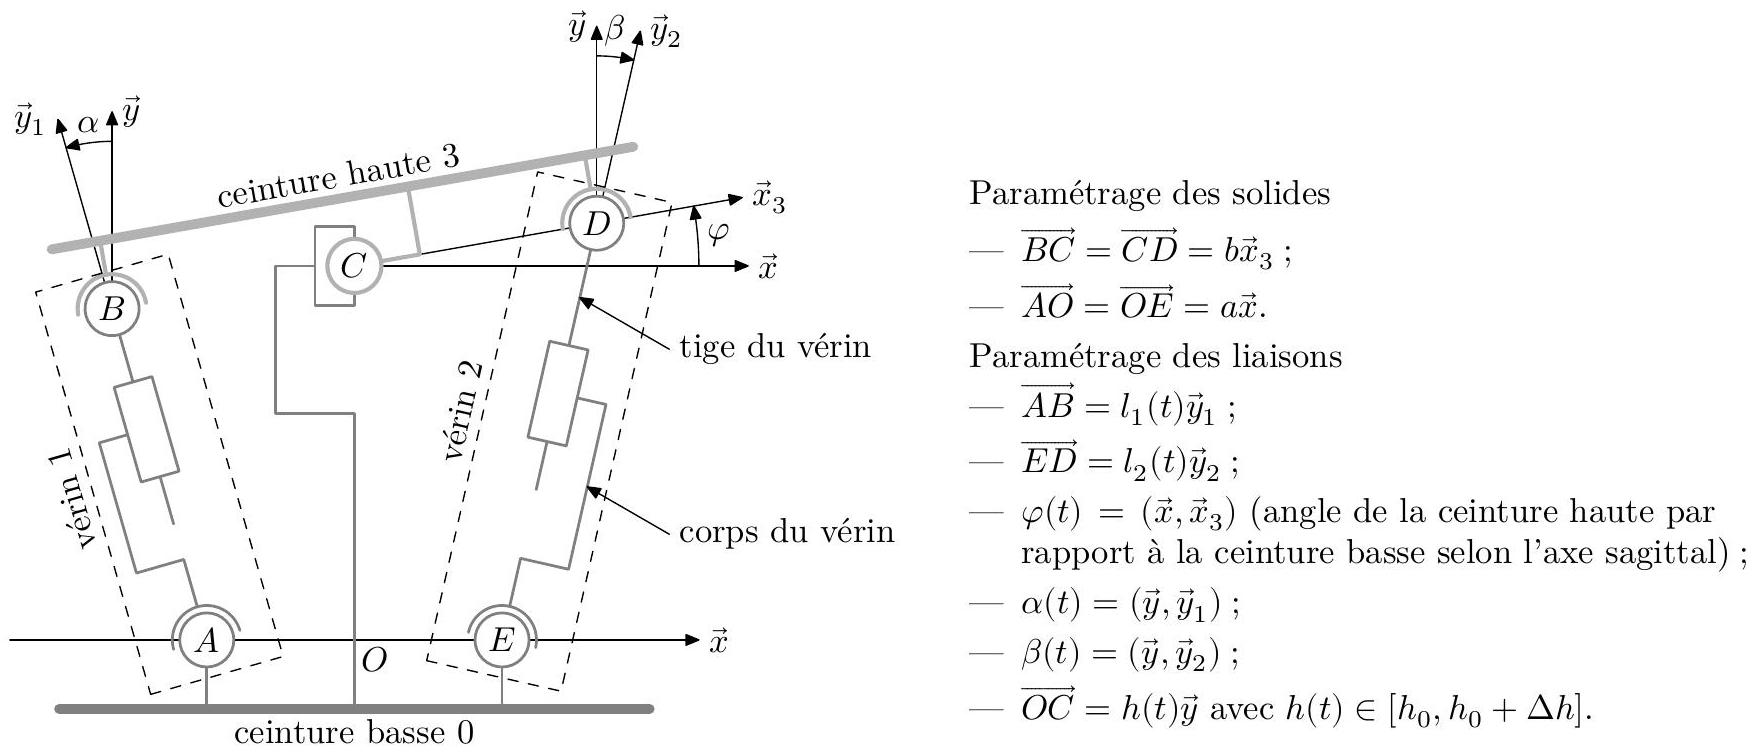
\includegraphics[width=\textwidth]{2025_09_16_5f2d7643f7e649c6833dg-05(1)}
%\captionsetup{labelformat=empty}
%\caption{Figure 7 Paramétrage cinématique}
%\end{center}
%\end{figure}


\begin{figure}[!h]
\centering
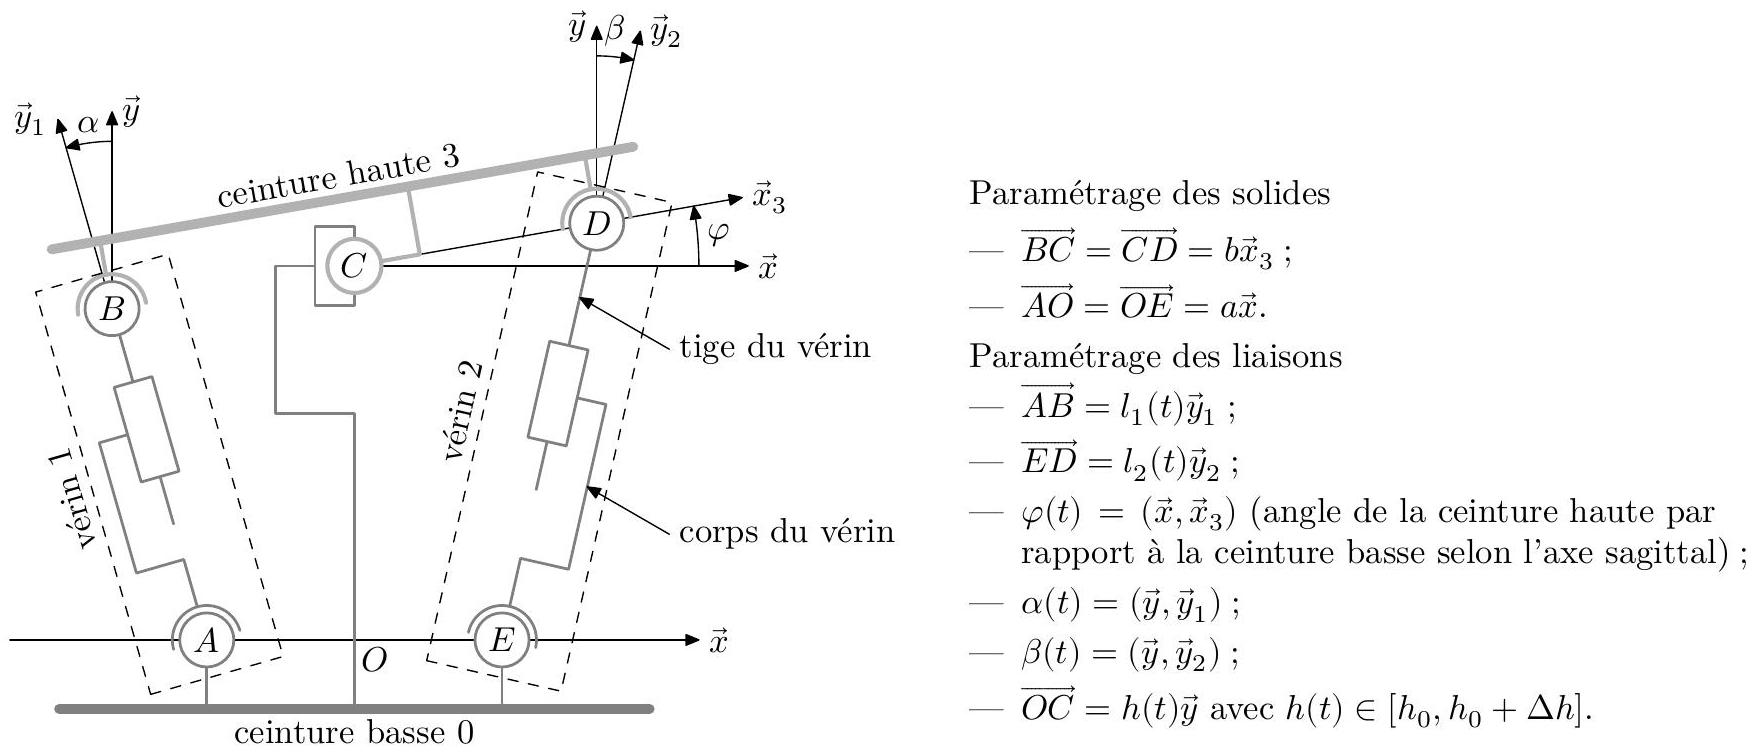
\includegraphics[width=\textwidth]{2025_09_16_5f2d7643f7e649c6833dg-05(1)}
\caption{\label{ccs_mp_2023_fig_07} Paramétrage cinématique }
\end{figure}




Le protocole de mise en précontrainte et d'utilisation de l'exosquelette est le suivant:

\begin{enumerate}
  \item à $t=0$, mise en place de l'ensemble en ajustant sur le corps de l'usager les deux ceintures basse et haute $\left(h_{0}=h(0)\right)$;
  \item pour $t \in[0, T]$, mise en précontrainte $\left(h(T)=h_{0}+\Delta h\right)$;
  \item pour $t>T$, mouvement libre (dans notre étude, $\varphi(t)$ est limité de $0^{\circ}$ à $20^{\circ}$ selon l'axe sagittal).
\end{enumerate}

On définit la course d'un actionneur linéaire comme étant la distance que peut parcourir la tige par rapport au corps entre ses positions extrêmes.\\

%Q 4. 
\question{\label{ccs_mp_2023_q_04}
Le point $C$ restant sur l'axe $\axe{O}{y}$, déterminer la course du vérin 2 à partir du protocole défini précédemment pour les valeurs $a=100 \mathrm{~mm}, b=150 \mathrm{~mm}, h_{0}=100 \mathrm{~mm}$ et $\Delta h=50 \mathrm{~mm}$.}
\ifprof
\begin{corrige}
\end{corrige}
\else
\fi


Une étude équivalente montre que la course du vérin 2 est supérieure à celle du vérin 1 .

La course obtenue permet donc de dimensionner géométriquement les actionneurs en fonction des positions des points d'accroche sur les ceintures haute et basse. On peut ainsi définir la valeur de contrôle à mettre en place sur le banc d'essai. Cette valeur est vérifiée pour chaque actionneur fabriqué.\\
L'exigence sur la liberté de mouvement angulaire étant vérifiée, la suite de l'étude a pour but de caractériser la dynamique et la commande d'un des quatre actionneurs ce qui nécessite l'élaboration d'un modèle de connaissance. La validation sera faite à partir des résultats de la force de traction mesurée sur le banc d'essai.


%%%% DEBUT AJOUT %%%
\subsection{Analyse de la structure cinématique de l'exosquelette} % Ajout XP

\question{Tracer le graphe des liaisons associé au modèle d'exosquelette proposé figure \ref{ccs_mp_2023_fig_07}.}

\question{\textbf{Sans calcul}, proposer une méthode permettant de déterminer la liaison équivalente entre la ceinture basse \textbf{0} et la ceinture haute \textbf{3}.}

On donne ci-dessous les figures planes permettant de paramétrer les angles de la liaison sphérique de centre $A$.

\question{Exprimer le torseur cinématique de la liaison équivalente entre le solide 3 et le solide 0 en passant par le vérin 1 au point $B$. Exprimer ensuite le torseur de la liaison des actions mécaniques.}

\question{Déterminer la liaison équivalente entre le solide 3 et le solide 0. En déduire le nombre de mobilités utiles du modèle.}



\question{Déterminer méthodiquement le degré d'hyperstisme du modèle proposé figure \ref{ccs_mp_2023_fig_07}.}




